\chapter{Similarity Renormalization Group Formalism}\label{srg_formalism}

In this chapter, we introduce the physics concepts and formalism necessary to understand the 1-dimensional problems to which SRG is applied. We then introduce SRG and discuss details and open questions regarding its use.

\section{Quantum Mechanics Operators}

Operators in quantum mechanics act linearly on state vectors, which represent specific states of the system. Each operator corresponds to some physical quantity; for example, the Hamiltonian, $\hat{H}$, which is the sum of kinetic and potential energy operators, $\hat{T}$ and $\hat{V}$ respectively, is connected with the possible energies of the system. A state, which in Dirac notation is denoted by an abstract ket, $\ket{\Psi}$, is said to be an eigenstate with eigenvalue $\omega$ of some operator, $\hat{\Omega}$, when the following equation holds:
\begin{equation}
\hat{\Omega}\ket{\Psi} = \omega\ket{\Psi}.
\end{equation}
These eigenvalues are the \textit{observables} (i.e. measurable quantities) of quantum mechanical systems.

Operators exist in a Hilbert space spanned by a basis of state vectors, $\ket{\Psi_i}$. An operator's representation with respect to a basis is given by its matrix elements,
\begin{equation}
\hat{\Omega}_{ij} = \bra{\Psi_i}\Omega\ket{\Psi_j}.
\end{equation}
An operator can be transformed to a different basis through a unitary transformation, which preserves its eigenvalues and thus its observables. Examples of 1-dimensional single-particle bases include particle position, $x$, particle momentum, $p$, and the 1-dimensional harmonic oscillator basis, which will be discussed next.

\subsection{1-Dimensional Harmonic Oscillator}

\begin{figure}[t]
\begin{center}
\subfloat[\label{fig:ho_wf_w_1}]{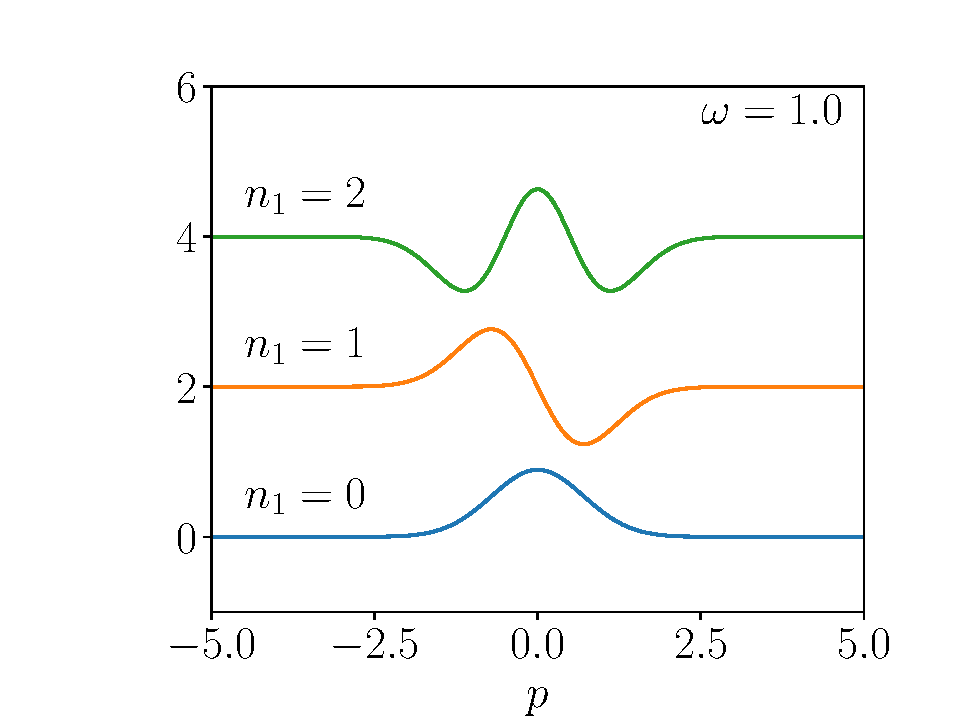
\includegraphics[width=0.5\linewidth]{ho_plot_1}}
\subfloat[\label{fig:ho_wf_w_4}]{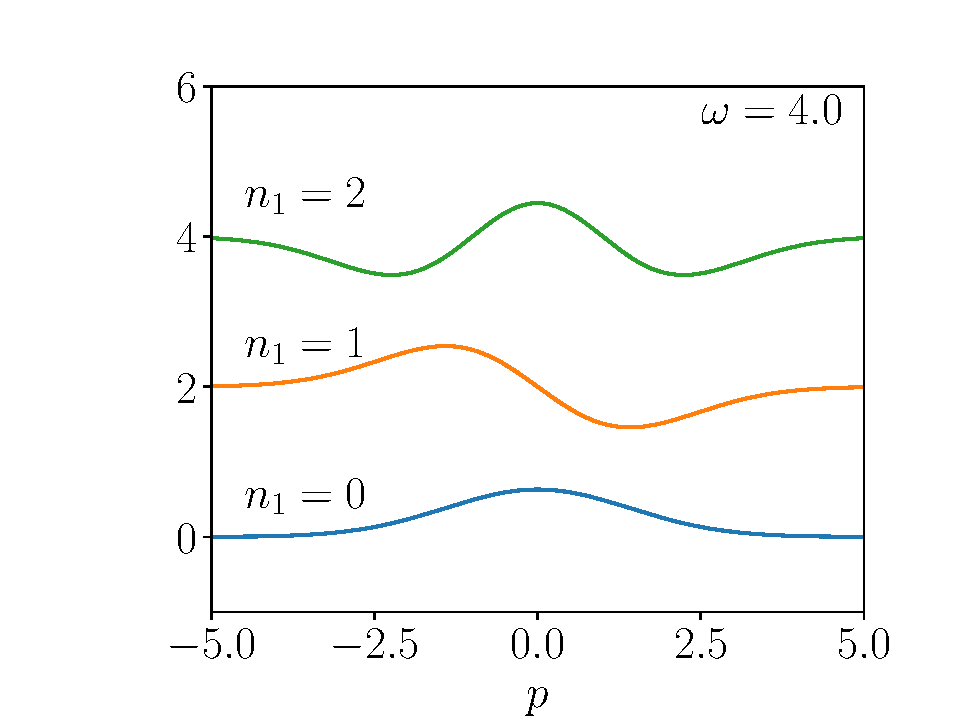
\includegraphics[width=0.5\linewidth]{ho_plot_4}}
\end{center}
\caption{1-dimensional harmonic oscillator wavefunctions for the three lowest energy states for (a) $\omega=1$ and (b) $\omega=4$.}
\label{fig:ho_wf}
\end{figure}

The 1-dimensional harmonic oscillator is a single particle in a purely quadratic potential, $\hat{V}(x) = m\omega^2 \hat{x}^2/2$. The Hamiltonian for the quantum harmonic oscillator is given by
\begin{equation}
\hat{H}_{HO} = \frac{\hat{p}^2}{2m} + \frac{1}{2}m\omega^2\hat{x}^2,
\end{equation}
which has eigenstates $\ket{n}$, which have corresponding wavefunctions
\begin{equation}
\Psi_n(x) = \frac{1}{\sqrt{2^n n!}}\left(\frac{m \omega}{\pi \hbar}\right)^{1/4}e^{-m \omega x^2 / 2 \hbar} H_n\left(\sqrt{\frac{m \omega}{\hbar}}x\right)
\end{equation}
\begin{equation}
\Phi_n(p) = \frac{(-i)^n}{\sqrt{2^n n!}}\left(\frac{1}{\pi m \hbar \omega}\right)^{1/4}e^{-p^2 / 2 m \hbar \omega} H_n\left(\frac{p}{\sqrt{m \omega \hbar}}\right)
\end{equation}
where $H_n(x)$ is the $n$-th Hermite polynomial. The three lowest energy momentum-space wavefunctions, $\Phi_n(p)$, can be seen in Fig.~\ref{fig:ho_wf}. The harmonic oscillator can also be rewritten as
\begin{equation}
\hat{H}_{HO} = \hbar \omega \left(\hat{a}^\dagger \hat{a} + \frac{1}{2}\right),
\end{equation}
where $\hat{a}^\dagger$ and $\hat{a}$ are raising and lowering operators which act on the harmonic oscillator eigenstates like
\begin{equation}
\hat{a}^\dagger\ket{n} = \sqrt{n + 1}\ket{n+1}
\end{equation}
\begin{equation}
\hat{a}\ket{n} = \sqrt{n}\ket{n-1}.
\end{equation}

For an operator, $\hat{V}$, represented with respect to a momentum basis, $V(p, p')$, a transformation to a harmonic oscillator basis can be achieved by the following calculation:
\begin{equation}\label{eq:ho_transform}
\bra{n}\hat{V}\ket{n'} = \iint V(p, p') \Phi_n^*(p) \Phi_{n'}(p') \,dp\,dp'.
\end{equation}

\subsection{Many-particle states}

For a system of $A$ non-interacting particles, the energy eigenstates of the system can be written as a product of the eigenstates of the single particle Hamiltonians:
\begin{equation}
\ket{\Psi} = \prod_{i=1}^{A}\ket{\Psi_k}_i
\end{equation}
where $\ket{\Psi_k}_i$ is the $k$-th eigenstate of the $i$-th particle's single particle Hamiltonian. For $A$ non-interacting particles in a harmonic oscillator potential, these product states are denoted by:
\begin{equation}
\ket{n_1 n_2 ... n_A} = \prod_{i=1}^{A}\ket{n_i}_i.
\end{equation}


\section{1-Dimensional System of Bosons}

The Hamiltonian for a 1-dimensional system of $A$ identical bosons with mass $m$ that interact via a local two-body potential is as follows:
\begin{equation}
\hat{H} = \frac{1}{2 m} \sum_{i=1}^A \hat{k}_i^2 + \sum_{i=1}^A\sum_{j=i+1}^{A} \hat{V}(x_i - x_j).
\end{equation}
In this equation, the $\hat{k}_i$ are the single-particle momenta and the $x_i$ are the single-particle coordinates. A local potential is a function of the distance between two particles, as opposed to a function of both of their absolute coordinates.

\subsection{Jacobi Coordinates}

A factorization of the Hamiltonian into a center-of-mass component, which is unaffected by the local potential, and a component relative to the center of mass is possible. This is achieved by a transformation to relative momentum Jacobi coordinates. These are defined to be:
\begin{equation}
p_i = \sqrt{\frac{i}{i+1}} \left(\frac{1}{i} \sum_{j=1}^{i}(k_j - k_{i+1})\right),
\end{equation}
with $k_i$ being the single-particle momenta as mentioned above. It is worth noting that for a system of $A$ particles, we only need $A-1$ Jacobi momentum coordinates. We can get $\hat{V}$ in terms of incoming Jacobi momentum $p$ and outgoing momentum $p'$ by taking the following Fourier transform of $\hat{V}(x_1 - x_2)$
\begin{equation}
\hat{V}(p, p') = \int \hat{V}(\sqrt{2} l_1) e^{- i (p - p') l_1} \,dl_1,
\end{equation}
where $l_1$ is the coordinate conjugate of $p_1$, $(x_1 - x_2)/\sqrt{2}$. Removing the center-of-mass component of the Hamiltonian, we find the new Hamiltonian to be
\begin{equation}
\hat{H} = \frac{1}{2 \mu} \sum_{i=1}^{A-1} \hat{p}_i^2 + \sum_{i=1}^{A-1}\hat{V}(p_i, p_i'),
\end{equation}
where $\mu$ is the reduced mass given by $\mu = m / A$ for particles of equal mass. For the purposes of this work, we will be starting with a potential defined with respect to the Jacobi momentum coordinates, avoiding the process of Fourier transforming a local coordinate-space potential.

\subsection{Transformation To Harmonic Oscillator States}

In momentum space, SRG evolutions require separate treatment of 2-body, 3-body, and higher-body potentials, to avoid delta functions caused by spectator particles. A particle is a spectator particle when it is in a state where it does not interact with two particles that are interacting with each other. To avoid the cognitive load of handling all these potentials separately, we can make a transformation to a discrete basis. The discrete basis of choice for this project is the harmonic oscillator basis with respect to the Jacobi coordinates. This transformation can be achieved as shown in Eq.~\ref{eq:ho_transform}. From here on out, $\ket{n_i}$ will mean the $n$-th harmonic oscillator state with respect to the $i$-th Jacobi coordinate. So for a full treatment of an $N$-particle system, we will need product states for $N-1$ Jacobi coordinates,
\begin{equation}
\ket{n_1 n_2 ... n_{A-1}} = \prod_{i=1}^{A-1}\ket{n_i}.
\end{equation}

\subsection{Symmetrizing the Harmonic Oscillator Basis}

According to the spin-statistics theorem, the state of a system of bosons must be symmetric under any permutation of the particle coordinates. We approach the problem of generating a basis of states that reflect this symmetry recursively, by first symmetrizing the 2-body system and then going from a symmetrized $(A-1)$-body basis to a symmetrized $A$-body basis. At each stage, we must diagonalize the symmetrizer, the form of which we will show for the 2-body and 3-body cases.

For the 2-particle system, we are only working with the first Jacobi coordinate and the harmonic oscillator states corresponding to it, $\ket{n_1}$. The symmetrizer is $\hat{S} = (1 + \hat{P}_{12})/2$, where $\hat{P}_{ij}$ is the operator that exchanges the coordinates between $i$-th and $j$-th particles. Because harmonic oscillator wavefunctions are either even for even $n$ or odd for odd $n$, $\hat{P}_{12} \ket{n_1} = (-1)^{n_1} \ket{n_1}$ and the symmetrizer is already diagonal with eigenvalue 0 for odd $n_1$ and eigenvalue 1 for even $n_1$. We select the states with eigenvalue 1 to create our symmetric harmonic oscillator basis for the 2-particle system.

To generate the partially symmetrized basis for the 3-body system, we take the states $\ket{n_1 n_2}$ where the possible $n_1$ values come from the symmetrized 2-body basis. The general 3-body symmetrizer is governed by the permutation group $S_3$, generated by $\hat{P}_{12}$ and $\hat{P}_{23}$, and has the form
\begin{equation}
\hat{S} = \frac{1}{6}(1 + \hat{P}_{12} + \hat{P}_{23} + \hat{P}_{23}\hat{P}_{12} + \hat{P}_{12}\hat{P}_{23}\hat{P}_{12})
\end{equation}
Since the states included in our to-be-symmetrized basis are already symmetric with respect to $\hat{P}_{12}$, the symmetrizer simplifies to $\hat{S} = (1 + 2\hat{P}_{23})/3$. The matrix elements of $\hat{P}_{23}$ in our partially symmetrized basis are
\begin{equation}
\bra{n_1' n_2'}\hat{P}_{23}\ket{n_1 n_2} = \delta_{N',N} \bra{n_1' n_2'}\ket{n_1 n_2}_3,
\end{equation}
where $N'=n_1' +n_2'$, $N=n_1 + n_2$, and $\bra{n_1' n_2'}\ket{n_1 n_2}_3$ is the 1-dimensional harmonic oscillator transformation bracket for particles with mass ratio 3. This transformation bracket value is calculated as
\begin{equation}
\bra{n_1' n_2'}\ket{n_1 n_2}_3 = \frac{\sqrt{n_1!n_2!}}{\sqrt{n_1'!n_2'!}}\sum_{k=0}^{n_1'}\binom{n_1'}{k}\binom{n_2'}{n_2 - k}\left(\frac{1}{2}\right)^{n_1' + n_2 - 2k}\left(\frac{\sqrt{3}}{2}\right)^{n_2' - n_2 + 2k} (-1)^{n_2-k}.
\end{equation}
Diagonalizing $\hat{S}$ will give eigenvectors that are normalized linear combinations of product states with the same total harmonic oscillator number $N$. We again select the ones with eigenvalue 1 and keep those as our fully symmetrized 3-body basis. While the project leading up to this thesis only worked with 2-particle and 3-particle systems and thus only the treatment of symmetrizing those bases is relevant to this work, the procedure is generalizable to symmetrize up to any $A$-particle basis. The details of this procedure are explained in Ref.~\cite{Jurgenson:2008jp}.

\subsection{Matrix Elements in the 3-Body Harmonic Oscillator Space}

From Eq.~\ref{eq:ho_transform}, we are able to transform both parts of our 2-body Hamiltonian into the symmetrized 2-body harmonic oscillator basis. In order to work in a symmetrized 3-body basis, we need to compute the kinetic energy for the 3-body system and embed the 2-body potential in the 3-body space. Both the $A$-body kinetic energy and the $A$-body embedded 2-body potential are defined with respect to their $(A-1)$-body counterparts, so we will set up the discussion to give those formulas. Let $\ket{N_A i_A}$ be a symmetrized $A$-body state with total harmonic oscillator number $N_A$ and degeneracy label $i_A$. $\ket{N_A i_A}$ is defined as
\begin{equation}
\ket{N_A i_A} = \sum_{l=1}^k c_l \ket{N_{A-1} i_{A-1}; n_{A-1}},
\end{equation}
where $k$ is the number of states in the linear combination, the $c_l$ are the coefficients of the linear combination of product states that make up the symmetrized state, $\ket{n_{A-1}}$ is a harmonic oscillator state with respect to the $(A-1)$-th Jacobi coordinate, and $\ket{N_{A-1} i_{A-1}}$ is a symmetrized $(A-1)$-body state. The $A$-body kinetic energy is calculated as
\begin{equation}
\begin{aligned}
\bra{N_A' i_A'}\hat{T_A}\ket{N_A i_A} = & \sum_{l=1}^k \sum_{l'=1}^{k'} c_l c_{l'}' (\bra{N_{A-1}' i_{A-1}'}\hat{T_{A-1}}\ket{N_{A-1} i_{A-1}}\delta_{n_{A-1}',n_{A-1}} \\ 
& + \frac{\omega}{4}\delta_{N_{A-1}',N_{A-1}}(\sqrt{(n_{A-1} + 1)(n_{A-1} + 2)}\delta_{n_{A-1}',n_{A-1} + 2} \\
& + \sqrt{n_{A-1}(n_{A-1} - 1)}\delta_{n_{A-1}',n_{A-1} - 2} \\
& - (2 n_{A-1} + 1)\delta_{n_{A-1}',n_{A-1}})).
\end{aligned}
\end{equation}
Similarly, the embedded 2-body potential in the $A$-body basis is calculated as
\begin{equation}
\bra{N_A' i_A'}\hat{V_A}\ket{N_A i_A} = \frac{A}{A-2} \sum_{l=1}^k \sum_{l'=1}^{k'} c_l c_{l'}' \bra{N_{A-1}' i_{A-1}'}\hat{V_{A-1}}\ket{N_{A-1} i_{A-1}}\delta_{n_{A-1}',n_{A-1}}.
\end{equation}

\section{Similarity Renormalization Group}

The similarity renormalization group (SRG), whose use in low-energy nuclear physics was initially explored at OSU, is one method of reducing the computational complexity of low-energy nuclear calculations. The idea behind it is to continuously unitarily transform the operator of interest (for example, the Hamiltonian) into a simpler form. This simpler form is chosen to allow the large basis to be truncated without affecting the operator eigenvalues, which are essential to the truncated operator's utility in later calculations. The SRG transformation is given by the flow equation for the evolving Hamiltonian $H_s$,
\begin{equation}
\frac{d \hat{H}_s}{ds} = [\hat{\eta}_s, \hat{H}_s],
\end{equation}
where $[A, B]$ is the matrix commutator and $\hat{\eta}_s$ is the generator of the transformation which is defined as
\begin{equation}
\hat{\eta}_s = [\hat{G}_s, \hat{H}_s],
\end{equation}
where $\hat{G}_s$ is known as the flow operator. The changes in the Hamiltonian over the course of the SRG evolution are absorbed into the potential, $\hat{V}_s$, leaving the kinetic energy, $\hat{T}$, independent of $s$, the flow parameter. $s$ is taken to be 0 for the un-evolved Hamiltonian. It is often convenient to use $\lambda = 1 / s^{1/4}$ as an alternative flow parameter, so instead of going from $s=0$ towards $s=\infty$ over the course of an SRG transformation, you are going from $\lambda=\infty$ towards $\lambda=0$. For our purposes, $\lambda=40$ (or $s=3.9 \times 10^{-7}$) will be a good enough place to start with the initial Hamiltonian.

\subsection{Induced Many-Body Forces and Flow Operators}

The SRG evolution is fully unitary for an $A$-body operator when done in the $A$-body space. However, working in the full many-body space is only feasible for the smallest of systems, due to the combinatorial scaling of the basis size with respect to $A$. When evolving an $A$-body system operator in some smaller basis, the SRG evolution induces many-body forces which show up as an error when eventually computing operator observables further down the line. This error has limited the SRG's domain of applicability to calculations for small to medium-sized systems.

Certain results have suggested that alternative choices for the flow operator, $\hat{G}_s$, could reduce this many-body force induction and thereby reduce the error induced by applying SRG to calculations \cite{Dicaire:2014fra}. The standard choice for $\hat{G}_s$ is the kinetic energy, which is easy to calculate and represent in most problems. Alternative flow operator choices have been explored previously, but not thoroughly.

\subsection{Value of the 1-Dimensional Laboratory}

SRG was explored initially in the 1-dimensional setting, which made it easy to test and allowed those exploring it to learn a great deal, such as the more careful treatment necessary for $A$-body evolutions in momentum space. Moreover, the setup of the 1-dimensional system is analogous to that of more complex calculations, so the results from the 1-dimensional setting generalize to application of the SRG in 3-dimensional calculations. If there is something to be learned about the connection between flow operator and many-body force induction, it is best comprehensively explored in a simple 1-dimensional problem and then generalized to expensive, difficult 3-dimensional calculations.

We will now explain the structure of the Python framework designed to make it easy to explore SRG in this 1-dimensional setting.